\documentclass[journal, a4paper]{IEEEtran}

% some very useful LaTeX packages include:

%\usepackage{cite}      % Written by Donald Arseneau
% * <yueguo@iu.edu> 2018-09-01T13:39:33.474Z:
%
% ^.
                        % V1.6 and later of IEEEtran pre-defines the format
                        % of the cite.sty package \cite{} output to follow
                        % that of IEEE. Loading the cite package will
                        % result in citation numbers being automatically
                        % sorted and properly "ranged". i.e.,
                        % [1], [9], [2], [7], [5], [6]
                        % (without using cite.sty)
                        % will become:
                        % [1], [2], [5]--[7], [9] (using cite.sty)
                        % cite.sty's \cite will automatically add leading
                        % space, if needed. Use cite.sty's noadjust option
                        % (cite.sty V3.8 and later) if you want to turn this
                        % off. cite.sty is already installed on most LaTeX
                        % systems. The latest version can be obtained at:
                        % http://www.ctan.org/tex-archive/macros/latex/contrib/supported/cite/

\usepackage{graphicx}   % Written by David Carlisle and Sebastian Rahtz
                        % Required if you want graphics, photos, etc.
                        % graphicx.sty is already installed on most LaTeX
                        % systems. The latest version and documentation can
                        % be obtained at:
                        % http://www.ctan.org/tex-archive/macros/latex/required/graphics/
                        % Another good source of documentation is "Using
                        % Imported Graphics in LaTeX2e" by Keith Reckdahl
                        % which can be found as esplatex.ps and epslatex.pdf
                        % at: http://www.ctan.org/tex-archive/info/

%\usepackage{psfrag}    % Written by Craig Barratt, Michael C. Grant,
                        % and David Carlisle
                        % This package allows you to substitute LaTeX
                        % commands for text in imported EPS graphic files.
                        % In this way, LaTeX symbols can be placed into
                        % graphics that have been generated by other
                        % applications. You must use latex->dvips->ps2pdf
                        % workflow (not direct pdf output from pdflatex) if
                        % you wish to use this capability because it works
                        % via some PostScript tricks. Alternatively, the
                        % graphics could be processed as separate files via
                        % psfrag and dvips, then converted to PDF for
                        % inclusion in the main file which uses pdflatex.
                        % Docs are in "The PSfrag System" by Michael C. Grant
                        % and David Carlisle. There is also some information
                        % about using psfrag in "Using Imported Graphics in
                        % LaTeX2e" by Keith Reckdahl which documents the
                        % graphicx package (see above). The psfrag package
                        % and documentation can be obtained at:
                        % http://www.ctan.org/tex-archive/macros/latex/contrib/supported/psfrag/

%\usepackage{subfigure} % Written by Steven Douglas Cochran
                        % This package makes it easy to put subfigures
                        % in your figures. i.e., "figure 1a and 1b"
                        % Docs are in "Using Imported Graphics in LaTeX2e"
                        % by Keith Reckdahl which also documents the graphicx
                        % package (see above). subfigure.sty is already
                        % installed on most LaTeX systems. The latest version
                        % and documentation can be obtained at:
                        % http://www.ctan.org/tex-archive/macros/latex/contrib/supported/subfigure/

\usepackage{url}        % Written by Donald Arseneau
                        % Provides better support for handling and breaking
                        % URLs. url.sty is already installed on most LaTeX
                        % systems. The latest version can be obtained at:
                        % http://www.ctan.org/tex-archive/macros/latex/contrib/other/misc/
                        % Read the url.sty source comments for usage information.

%\usepackage{stfloats}  % Written by Sigitas Tolusis
                        % Gives LaTeX2e the ability to do double column
                        % floats at the bottom of the page as well as the top.
                        % (e.g., "\begin{figure*}[!b]" is not normally
                        % possible in LaTeX2e). This is an invasive package
                        % which rewrites many portions of the LaTeX2e output
                        % routines. It may not work with other packages that
                        % modify the LaTeX2e output routine and/or with other
                        % versions of LaTeX. The latest version and
                        % documentation can be obtained at:
                        % http://www.ctan.org/tex-archive/macros/latex/contrib/supported/sttools/
                        % Documentation is contained in the stfloats.sty
                        % comments as well as in the presfull.pdf file.
                        % Do not use the stfloats baselinefloat ability as
                        % IEEE does not allow \baselineskip to stretch.
                        % Authors submitting work to the IEEE should note
                        % that IEEE rarely uses double column equations and
                        % that authors should try to avoid such use.
                        % Do not be tempted to use the cuted.sty or
                        % midfloat.sty package (by the same author) as IEEE
                        % does not format its papers in such ways.

\usepackage{amsmath}    % From the American Mathematical Society
                        % A popular package that provides many helpful commands
                        % for dealing with mathematics. Note that the AMSmath
                        % package sets \interdisplaylinepenalty to 10000 thus
                        % preventing page breaks from occurring within multiline
                        % equations. Use:
%\interdisplaylinepenalty=2500
                        % after loading amsmath to restore such page breaks
                        % as IEEEtran.cls normally does. amsmath.sty is already
                        % installed on most LaTeX systems. The latest version
                        % and documentation can be obtained at:
                        % http://www.ctan.org/tex-archive/macros/latex/required/amslatex/math/

\usepackage{bm}
\usepackage{booktabs}

% Other popular packages for formatting tables and equations include:

\usepackage{array}
% Frank Mittelbach's and David Carlisle's array.sty which improves the
% LaTeX2e array and tabular environments to provide better appearances and
% additional user controls. array.sty is already installed on most systems.
% The latest version and documentation can be obtained at:
% http://www.ctan.org/tex-archive/macros/latex/required/tools/

% V1.6 of IEEEtran contains the IEEEeqnarray family of commands that can
% be used to generate multiline equations as well as matrices, tables, etc.

% Also of notable interest:
% Scott Pakin's eqparbox package for creating (automatically sized) equal
% width boxes. Available 
% http://www.ctan.org/tex-archive/macros/latex/contrib/supported/eqparbox/

% *** Do not adjust lengths that control margins, column widths, etc. ***
% *** Do not use packages that alter fonts (such as pslatex).         ***
% There should be no need to do such things with IEEEtran.cls V1.6 and later.
\usepackage{listings}

% Your document starts here!
\begin{document}

% Define document title and author
	\title{E511-Signal Processing-Final Project}
	\author{Jonathan Branam, Jamie Israel, Jinju(Hellen) Jiang}
	\date{December, 13 2018}
	\maketitle
%
% ^.
% Write abstract here
\begin{abstract}
In this project we evaluated and implemented state of the art techniques to solve the monaural speech separation (diarization) problem using a variety of approached. We investigated classification, masking, and deep learning approaches to separate a generated set of mixed speech recordings.
\end{abstract}

% Each section begins with a \section{title} command
\section{Introduction}
There have been several recent developments in the use of deep learning to perform speaker diarization, or separation of multiple speech signals from a single source into separate homogeneous signals representing each individual speaker. This task is particularly challenging where the input is monophonic, there is no control over environmental conditions, the number of speakers is unknown and there are no samples of the speakers from which to train. Using the CSR-I(WSJ0) Complete dataset\cite{garofolo:wsj0}, we tested several algorithms for accomplishing monaural speech separation including classification (KMeans), various masking approaches (NMF, Ideal Ratio Mask[IRM], and complex Ideal Ratio Mask [cIRM]), and permutation-based deep learning approaches (Permutation Invariant Training [PIT] and utterance-level Permutation Invariant Training [uPIT]).

The motivating application is to separate agent and customer utterances from call center recordings, which involve short duration speech with occasional cross talk and at least one unknown speaker.

\section{Literature Review}

\subsection{Jamie's Lit Review}


\subsection{Deep Learning Approaches}

A seminal paper in applying deep learning to the task of speaker diarization was the Deep Clustering (DPCL) \cite{DBLP:journals/corr/HersheyCRW15} approach proposed by Hershey, et. al. They divided the task of separating source signals into two steps. The first step is to use a deep neural network to learn a set of embeddings that estimate a class-independent, low-rank pairwise affinity matrix. These embeddings are trained to minimize the distance between embeddings in the same partition while maximizing the distances between embeddings in different partitions. The partitions used in their technique do not include class labels so the model does not assign a particular class to each embedding. The resulting embeddings can then be separated using simple clustering algorithms such as $k$-means. This is in contrast to previous work that relies on \textit{spectral clustering} for segmentation which uses local affinity measures to optimize an objective function using spectral decomposition. The approach of Hershey, et. al. is typical in current research for deep learning: rather than using a complicated set of specially designed features, the deep clustering approach uses a deep neural network to discover the best features for producing the desired partitions.

This work is also important because it introduced a new training dataset for the task of monaural speech separation. The authors found that existing datasets were too limited in size or were not well fitted to their task. The deep learning techniques also require a large training set and so the authors adapted the Wall Street Journal (WSJ0) \cite{garofolo:wsj0} single-channel speaker corpus to produce a new dataset called WSJ0-2mix \cite{WSJmix} that was used by the later literature for comparison with DPCL.

The Deep Clustering technique achieved Signal-to-Distortion (SDR) improvements of up to 6 dB which outperformed their baseline of an oracle NMF approach of 5 dB SDR which was trained on the clean speaker sources. It is worth noting the these initial results were improved to 10.3 dB by further optimization of the model by using a deeper architecture, a longer temporal context, and improving the regularization of the network by \cite{DBLP:journals/corr/IsikRCWH16}. This advancement shows the improvements possible by tuning hyper-parameters of a deep learning model when applied to the task of speaker diarization.

One of the biggest problems plaguing deep learning techniques in source separation is the \textit{label permutation problem} which is that most separation algorithms must provide the reference magnitudes to the output layers of the network to compute the error. The ordering of these source streams is ambiguous and imposes an outside and unnecessary constraint on the training process. Note that DPCL, discussed above, avoids this problem due to its treatment of the source separation problem as a partitioning problem. Although DPCL was successful, it made a simplifying assumption that each time-frequency bin was assigned to a single speaker (determined by the results of clustering). In \cite{DBLP:journals/corr/YuKTJ16} Yu, et. al. proposed a new technique called permutation invariant training (PIT) that avoids the label ambiguity problem by treating the reference source streams as a set rather than an ordered list. One key innovation of PIT is to directly train on all possible permutations of sources ($S!$ possible assignments) and to compute the combined pairwise MSE for every assignment between each reference and the estimated source. PIT then directly minimized the MSE of the assignment with the lowest total MSE of every permutation. This means that the model is directly trained on label assignment and error evaluation.

PIT operates on a sequence of $N$ input frames termed a \textit{meta-frame} in order to make use of the available contextual information in the sequence. It also produces a window of frames as an output and minimizes the separation error at this meta-frame level. Since the input is shifted one (or more) frames and a new meta-frame is computed and the assignment is computed for each meta-frame, the output of PIT may produce different speaker assignments for each frame. This means that, although the label permutation problem at training time has been resolved, the output of PIT can still be improved by tracing the speaker assignments for each frame as a post-processing step.

The results of PIT are impressive and exceed 10 dB SDR improvements for the DNN and CNN approaches with optimal speaker assignment. The ideal ratio mask (IRM) results indicate the best possible improvement and are only slightly better than PIT with 12.3 dB SDR. Optimal speaker assignment means that as a post-processing step the speaker assignment from PIT is improved by tracing the speakers across meta-frames and determining the optimal speaker assignment for each frame. This improves performance because the PIT method assumes that the output-speaker does not switch across frames. Without the optimal assignment the performance of PIT degrades from a high of 10.9 dB to 5.6 - 7.8 dB.


The authors of PIT improved their technique by proposing uPIT which is an enhancement to PIT that includes an utterance-level cost function which solves the speaker tracing problem by causing the Recurrent Neural Network (RNN) to align frames from a particular speaker to the same output stream. uPIT (like PIT) is also a much simpler model than other proposed deep learning algorithms and the trained networks have strong generalization performance to unseen data. In the original PIT algorithm the optimal permutation is computed for each meta-frame which can result in the assignment of speakers to output streams to switch during inference. With uPIT the optimal permutation is calculated across the entire utterance assuming the same assignment for all output frames. This works in practice by using recurrent neural networks such as deep LSTM (long short-term memory) RNNs and bi-directional LSTM RNNs. Since a recurrent neural network has access to data from past frames (and in a BLSTM information both the past and future frames are available) uPIT does not need to be trained on a meta-frame of $N$ stacked frames as PIT did.

The results of uPIT are similar to the performance of PIT with optimal speaker tracing. Using a BLSTM and a phase sensitive mask (PSM, also referred to as a cIRM - a complex ideal ratio mask) uPIT achieves results near 11 dB SDR. The maximum performance from the ideal PSM is about 15 dB SDR (an improvement over the 12.5 dB SDR possible with a standard IRM). Based on its performance and (relative) simplicity We chose uPIT as the deep learning solution that we evaluated in our project.


\section{Dataset Preparation}
\subsection{CSR-I (WSJ0) Complete}
For purposes of comparison with existing scholarship, each approach was developed based on a mixture of audio extracted from the WSJ0 dataset, a corpus of read speech texts drawn from articles in the Wall Street Journal. WSJ0 \cite{garofolo:wsj0} consists of over 35,000 audio samples organized into training and evaluation data sets organized by speaker and gender. The audio files are stored in a format called Sphere using the Shorten compression algorithm. The Linguistic Data Consortium website hosts a small utility called sph2pipe \cite{ldc:sph2pipe} which we used to convert the files from the Sphere format to waveform format. We wrote a small script to automate this process and also to merge the separate disks of the WSJ0 dataset into a single folder.

\subsection{WSJ0-mix}
The WSJ0-mix dataset was developed by the authors of the DPCL \cite{DBLP:journals/corr/HersheyCRW15} paper by mixing selections from the WSJ0 training set \texttt{si\_tr\_s} and mixing them together with different levels of signal-to-noise ratios (SNR) selected from 0 dB to 5dB. An additional cross validation was also generated from the training data and an evaluation set was generated with the same process but using the WSJ0 evaluation set \texttt{si\_et\_05} and development set \texttt{si\_dt\_05} which use different speakers than the training set. We found the definition of these mixtures and MATLABS scripts \cite{WSJmix} to produce the dataset from the WSJ0 data. We made some small adjustments to the scripts so that they would run in Octave, a free, open-source alternative to MATLAB, and to skip the step of generating 16 kHz outputs and the 3-speaker mixtures since we would not be using them.

The scripts produce 20,000 training files, 5,000 cross validation files, and 3,000 test files. Each of these includes the mixed audio as well as the independent sources which have had the correct SNR adjustments made to them. We further selected 1,000 training examples and 100 cross-validation and testing examples since we our algorithm was not able to finish running on the full dataset.


\section{Speech Separation Algorithms}
\subsection{KMeans}
The technique of speaker diarization relies on a big pipeline with following steps:
\begin{itemize}
    \item Feature Extraction
    \item Speaker segmentation
    \item Speaker Clustering
    \item Evaluation
\end{itemize}
\subsubsection{Feature Extraction}
In this project, we used 3 approaches to extract features:
\begin{itemize}
    \item A chroma vector (Wikipedia) (FMP, p. 123) is a typically a 12-element feature vector indicating how much energy of each pitch class, {C, C\#, D, D\#, E, ..., B}, is present in the signal. Then use mean of each element as one of input for clustering.
    \item The mel frequency cepstral coefficients (MFCCs) of a signal are a small set of features  which concisely describe the overall shape of a spectral envelope. In this case, mfcc computed 13 MFCCs.The very first MFCC, the 0th coefficient, does not convey information relevant to the overall shape of the spectrum. It only conveys a constant offset, i.e. adding a constant value to the entire spectrum. Therefore, here I discard the first MFCC, then I scale the MFCCs such that each coefficient dimension has zero mean and unit variance.Then use mean of MFCCS as one part of input for clustering.
    \item We divide the audio signal into smaller frames. In smaller time scales audio signals are statistically unchanged. Then for each smaller frames we compute the power spectrum of the signal, and use it as the third part of input for clustering.
\end{itemize}
\subsubsection{Speaker segmentation}\cite{Segmentation} Speaker segmentation which is also known as acoustic change detection aims to detect speaker change such that each contiguous segment corresponds to single speaker only. To find if the two segments correspond to same speaker we have to define some notion of distance metric. In this case, I skipped this step and used the features extrated from above steps as input for kmeans clustering.
\subsubsection{Kmeans Clustering}
Since we knew that the audio from call center is the conversation between 2 speakers(customer service and customer), we set k=2 for kmeans clustering.\\
here it is the results for speaker diarization.
\begin{figure}[h!]
    \centering  
     \caption{\label{Fig:speaker diarization}2 speakers diarization}  
    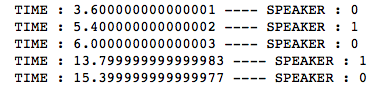
\includegraphics[width=0.4\textwidth]{kmeans01.png} 
\end{figure}

\begin{figure}[h!]
    \centering  
     \caption{\label{Fig:speaker diarization}2 speakers diarization}  
    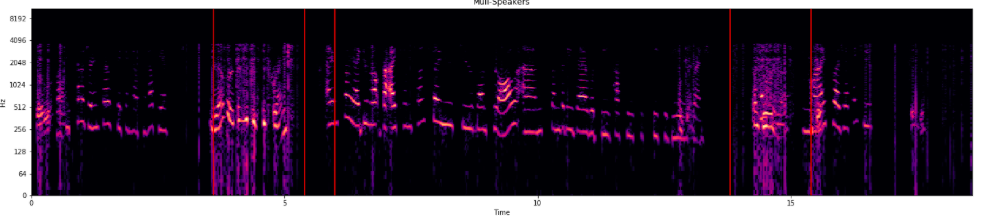
\includegraphics[width=0.4\textwidth]{kmeans02.png}
\end{figure}
\subsubsection{Evaluation\cite{Segmentation}}Diarization Error Rate (DER) is used for evaluation of automatic speech recognition system.Contribution to DER comes from three factors namely, Missed speech rate (MSR), False alarm speech rate (FASR) and Speaker Error. When a speech is labeled as non-speech then that error comes under MSR. FASR is when a non- speech is detected as a speech segment. Speaker error is contributed due to speaker clustering and segmentation. This kind of error can be caused if a speaker change is not detected, oversegmentation, erroneously clustered. Sum of all three errors contribute to the DER.\\
In this case, we don't have any labeled data to calculate the training error, we just simply used human ears to justify whether the diarization was good or not. For some training data, it works well, but some training data, it performed really bad. 

\subsection{NMF, IRM and cIRM}
Nonnegative matrix factorization (NMF) is used to represent high-dimensional data as the product of two matrices (typically referenced as $W$ and $H$). In the case of an audio signal, these matrices can be viewed as a representation of the signal's frequency spectrum ($W$) and the corresponding activations ($H$).

To perform NMF, we transformed isolated audio samples of two speakers (speaker 1 and speaker 2) to a frequency-time representation using short-time Fourier transform (STFT) before decomposing each signal using the following iterative update rules:
\newline

$W = W \bigodot \frac{\frac{X}{WH}H^T}{1{FxT}H^T}$ \hspace{1cm} $H = H \bigodot \frac{W^T\frac{X}{WH}}{W^T1^{FxT}}$
\newline

Using the frequency matrices associated with the sample from each speaker, a new set of activations ($W$) was generated from the mixed signal composed of both individual samples. A magnitude masking matrix, reflecting the magnitudes associated with the frequency representation for each speaker at each time frame, was generated using this new set of activations and the following formula:


\[
\dfrac{W_{S1}H_{(1:30,:)}}
{W_{S1}H_{(1:30,:)}+W_{S2}H_{(31:60,:)}}
\]

\begin{flushleft}
where S1 is the basis vector associated with the speaker 1 audio sample, S2 is the basis vector associated with the speaker 2 audio sample and H is the activation matrix generated from the combined speaker 1 and speaker 2 basis vectors.\cite{ClassNMF}
\end{flushleft}

Using the STFT of a single speaker audio sample (speaker 1) and the STFT of the mixed audio sample that included speaker 1 (Figure \ref{fig:spec_speaker_1}), an IRM was generated based on the formula:

\[
\dfrac{S_{(t,f)}^2}{S_{(t,f)}^2 + N_{(t,f)}^2}
\]

\begin{flushleft}

where $S$ is the STFT generated from the isolated speaker 1 audio signal and $N$ is the STFT generated from the mixed audio signal that included the same audio sample of speaker 1.\cite{DBLP:journals/corr/abs-1708-07524}

\end{flushleft}

\begin{figure}[h!]
    \centering  
     \caption{\label{fig:spec_speaker_1}Spectrogram of isolated and mixed audio sample from speaker 1}  
    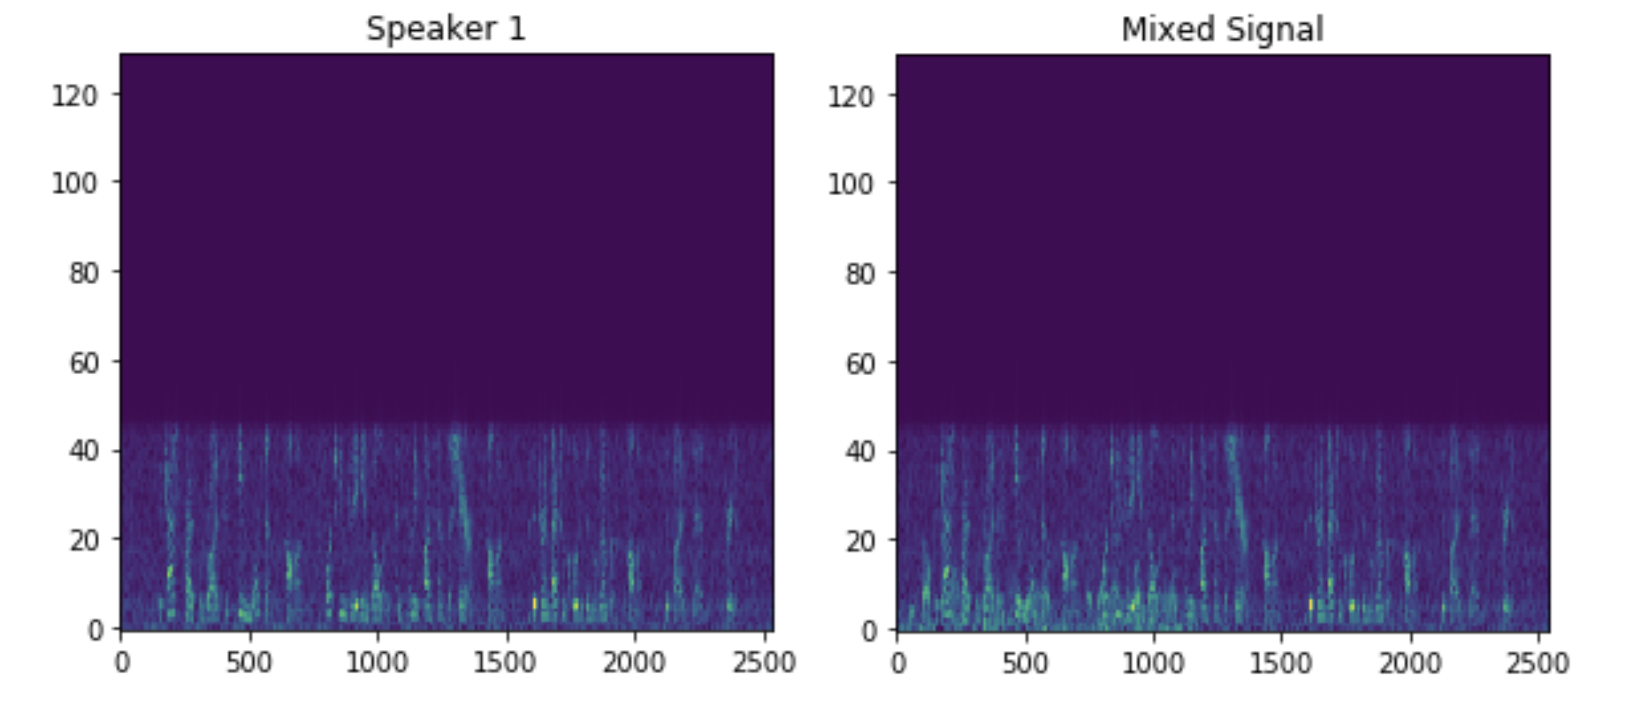
\includegraphics[width=0.4\textwidth]{cIRM_same.png}  
\end{figure}

Similarly, a cIRM was generated from the audio sample of speaker 1 and the same mixed audio sample using the formula:

\[
\dfrac{Y_r S_r + Y_i S_i}{Y_r^2 + Y_i^2} +
i\dfrac{Y_r S_i - Y_i S_r}{Y_r^2 + Y_i^2}
\]

\begin{flushleft}
where $S$ is the complex STFT representation generated from the isolated speaker 1 audio signal and $Y$ is the complex STFT generated form the mixed audio signal that included the same audio sample of speaker 1.\cite{DBLP:journals/corr/abs-1708-07524}
\end{flushleft}

\subsection{PIT and uPIT}

..
.... Add text here....


\section{Results}

\subsection{Masking Methods}

With the NMF method, we were unable to generate a substantial separation between the original isolated signal and the mixed audio. Both IMR approaches produced substantially better results with the cIMR method proving to be the best method for this type of separation on a consistent basis [Figure \ref{tab:masking_snr}].


\begin{figure}[h!]
    \centering  
     \caption{\label{Fig:Comparison of Average SNR for Masking Methods 1}Comparison of Average SNR for Masking Methods}  
    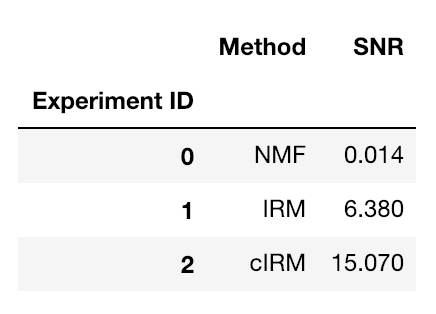
\includegraphics[width=0.3\textwidth]{Mask_Res.png}  
\end{figure}

\begin{table}[h]
    \centering
    \begin{tabular}{r r r}
        Label &Waveform & Kurtosis \\

        \midrule
        0 & s.wav & 7.29 \\
        1 & x1.wav & 4.91 \\
        2 & x2.wav & 3.87 \\
        \midrule
    \end{tabular}
    \caption{Table Caption}
    \label{tab:masking_snr}
\end{table}



\section{Conclusion}
...
\newline 
% Now we need a bibliography:

\bibliographystyle{plain} % We choose the "plain" reference style
\bibliography{report} % Entries are in the "refs.bib" file


% Your document ends here!
\end{document}
